\chapter{पाँच इंद्रियाँ}\label{ch:g1:the-five-senses}

\omterm{def:g1:the-five-senses:sense}{आँखें} बंद करो और संसार ग़ायब नहीं होता: तुम्हें कक्षा अब भी सुनाई देती
है, पकते खाने की महक आती है, और नीचे कुरसी महसूस होती है। शरीर के पास
संसार तक पहुँचने के पाँच दरवाज़े हैं --- इंद्रियाँ --- और हर दरवाज़ा
शरीर का एक अंग है, जो दिन भर तुम्हारे लिए काम करता है।

\section{पाँच इंद्रियाँ, पाँच अंग}

\begin{definition}[इंद्रिय और ज्ञानेंद्रिय]\label{def:g1:the-five-senses:sense}
\emph{इंद्रिय}\index{इंद्रिय} वह रास्ता है जिससे शरीर संसार के बारे
में जानता है। हर इंद्रिय एक \emph{ज्ञानेंद्रिय}\index{ज्ञानेंद्रिय}
से काम करती है, यानी शरीर का वह भाग जो उसी काम के लिए बना है:
\begin{enumerate}
  \item \emph{दृष्टि}\index{दृष्टि} --- \emph{आँखें}\index{आँख}
        प्रकाश, रंग और आकार देखती हैं;
  \item \emph{श्रवण}\index{श्रवण} --- \emph{कान}\index{कान} ध्वनियाँ
        सुनते हैं;
  \item \emph{घ्राण}\index{घ्राण} --- \emph{नाक}\index{नाक} महक लेती
        है;
  \item \emph{स्वाद}\index{स्वाद} --- \emph{जीभ}\index{जीभ} भोजन
        चखती है;
  \item \emph{स्पर्श}\index{स्पर्श} --- पूरे शरीर पर फैली
        \emph{त्वचा}\index{त्वचा} खुरदरा और चिकना, गरम और ठंडा महसूस
        करती है।
\end{enumerate}
\end{definition}

\begin{example}[नाश्ता, इंद्रिय दर इंद्रिय]\label{ex:g1:the-five-senses:breakfast}
गरम चॉकलेट का एक कटोरा पाँचों को काम पर लगा देता है: \omterm{def:g1:the-five-senses:sense}{आँखें} भाप देखती
हैं, नाक कोको की महक लेती है, हाथों की \omterm{def:g1:the-five-senses:sense}{त्वचा} गरम कटोरा महसूस करती है,
\omterm{def:g1:the-five-senses:sense}{कान} चम्मच की खनक सुनते हैं, और जीभ --- सबसे अच्छा हिस्सा --- उसे चखती
है।
\end{example}

\begin{omfigure}
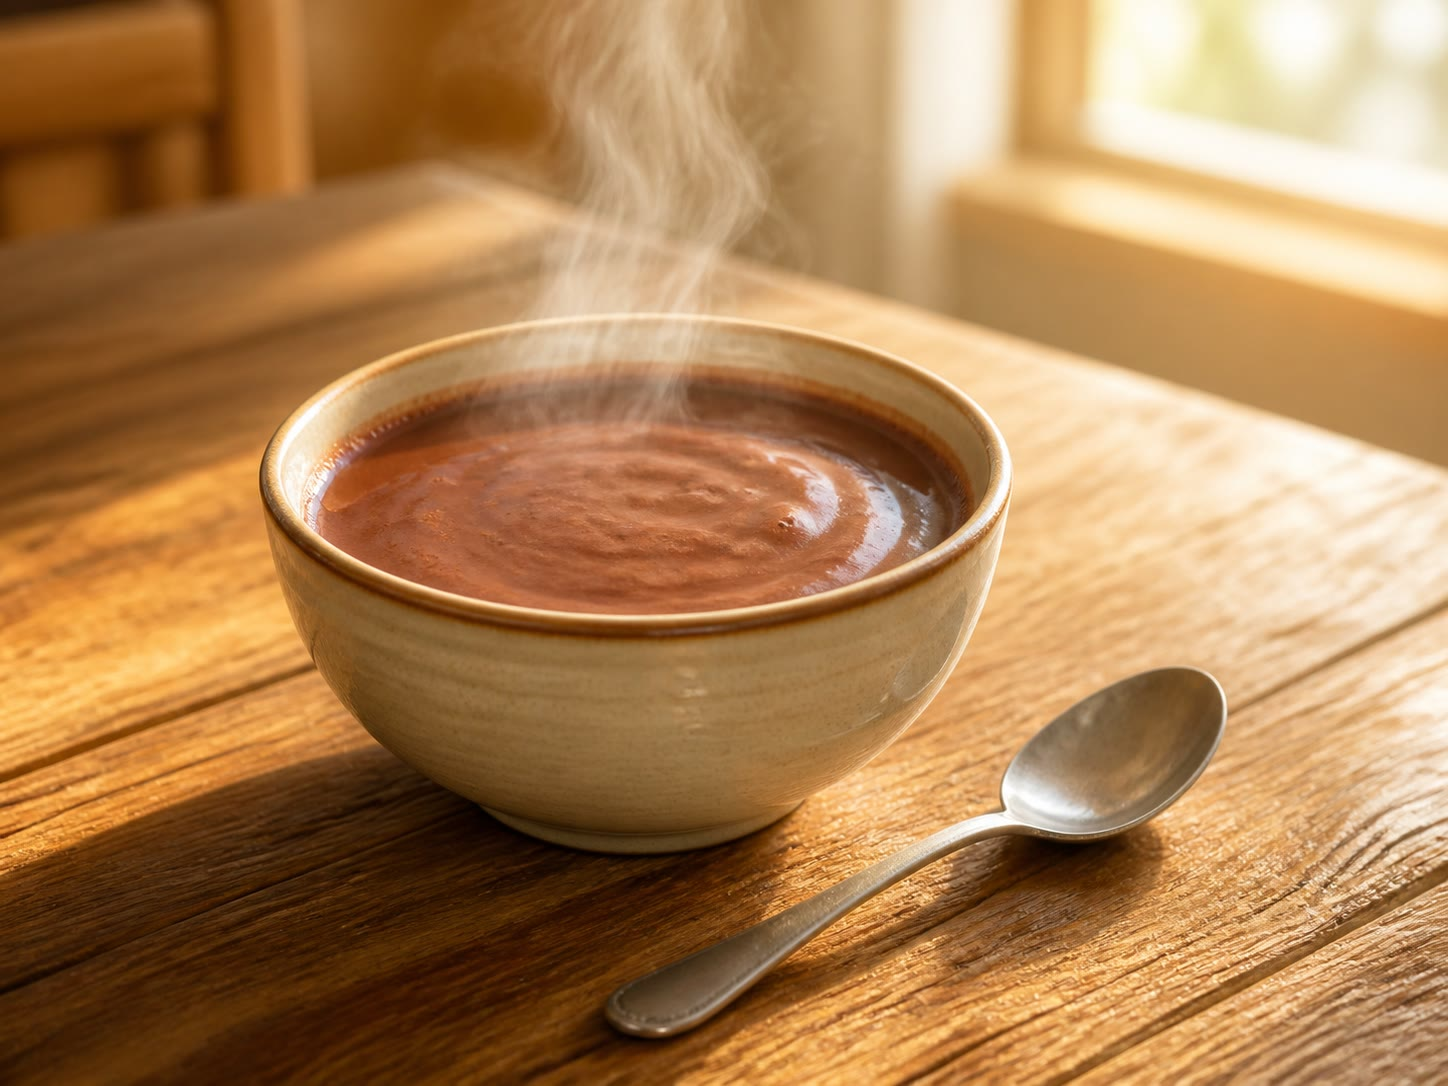
\includegraphics[width=0.58\linewidth]{images/book1/ai/g1-senses-chocolate.jpg}

{\small गरम चॉकलेट का एक कटोरा, और पहली चुस्की से पहले ही काम पर लगी
पाँचों इंद्रियाँ।}
\end{omfigure}

\begin{remark}[स्पर्श हर जगह है]\label{rem:g1:the-five-senses:skin}
चार ज्ञानेंद्रियाँ \omterm{def:g1:my-body:parts}{सिर} पर रहती हैं, पर स्पर्श का अंग \omterm{def:g1:the-five-senses:sense}{त्वचा} है, और
\omterm{def:g1:the-five-senses:sense}{त्वचा} तुम्हें \omterm{def:g1:my-body:parts}{सिर} से पाँव तक ढके रहती है। इसीलिए तुम गरदन पर हवा का
झोंका, जूते में कंकड़ और \omterm{def:g1:my-body:parts}{बाँह} पर बैठता गुबरैला महसूस कर लेते हो ---
वह भी बिना देखे।
\end{remark}

\section{इंद्रियाँ मस्तिष्क को ख़बर देती हैं}

\begin{proposition}[मस्तिष्क तक संदेश]\label{prop:g1:the-five-senses:brain}
\omterm{def:g1:the-five-senses:sense}{ज्ञानेंद्रिय} यह नहीं समझती कि उसने क्या भाँपा --- वह \emph{संदेश
भेजती है}। सारे संदेश शरीर के भीतर-भीतर \omterm{def:g1:my-body:parts}{सिर} में बैठे
\emph{मस्तिष्क}\index{मस्तिष्क} तक जाते हैं, जो उन्हें जोड़कर समझता
है: ``यह दादी की आवाज़ है'', ``यह महक टोस्ट की है''। मस्तिष्क के बिना
\omterm{def:g1:the-five-senses:sense}{आँखें} और \omterm{def:g1:the-five-senses:sense}{कान} किसी को ख़बर ही न दे पाते।
\end{proposition}
\admitted

\begin{omfigure}
\begin{tikzpicture}[scale=0.9]
  % brain box
  \draw[thick, omDef, fill=omDef!8, rounded corners=6pt]
    (4.6,0.2) rectangle (8.2,2.0);
  \node[font=\small\bfseries, omDef] at (6.4,1.55) {मस्तिष्क};
  \node[font=\small, align=center, text width=3.2cm] at (6.4,0.85)
    {संदेशों को\\ जोड़ता है};
  % organs
  \node[font=\small, left] (eye) at (2.2,2.6) {आँख देखती है};
  \node[font=\small, left] (ear) at (2.2,1.7) {कान सुनता है};
  \node[font=\small, left] (nose) at (2.2,0.8) {नाक महक लेती है};
  \node[font=\small, left] (skin) at (2.2,-0.1) {त्वचा महसूस करती है};
  % arrows
  \draw[->, thick, omMeth] (2.35,2.55) -- (4.55,1.75);
  \draw[->, thick, omMeth] (2.35,1.68) -- (4.55,1.35);
  \draw[->, thick, omMeth] (2.35,0.82) -- (4.55,0.95);
  \draw[->, thick, omMeth] (2.35,-0.02) -- (4.55,0.55);
  \node[font=\small, omMeth] at (3.4,3.0) {संदेश};
\end{tikzpicture}

{\small हर \omterm{def:g1:the-five-senses:sense}{ज्ञानेंद्रिय} अपना संदेश मस्तिष्क तक भेजती है, और मस्तिष्क
उन सबका अर्थ निकालता है। (जीभ भी ख़बर देती है --- बस चित्र भर जाता।)}
\end{omfigure}

\begin{example}[अँधेरे में नाम बताना]\label{ex:g1:the-five-senses:dark}
\omterm{def:g1:the-five-senses:sense}{आँखें} बंद रहते हुए कोई साथी तुम्हारे हाथ में जानी-पहचानी चीज़ रख देता
है: एक चाबी, एक स्पंज, एक चम्मच। तुम लगभग तुरंत उसका नाम बता देते हो।
\omterm{def:g1:the-five-senses:sense}{त्वचा} ने अपना संदेश भेजा --- ठंडी, सख़्त, नुकीली --- और मस्तिष्क ने
उत्तर दिया: ``चाबी''। इंद्रियाँ जुटाती हैं; मस्तिष्क समझता है।
\end{example}

\begin{remark}[एक-दूसरे की मदद]\label{rem:g1:the-five-senses:together}
इंद्रियाँ टोली बनाकर काम करती हैं। ज़ुकाम में नाक बंद हो तो खाना फीका
``लगता'' है, क्योंकि स्वाद का आधा काम तो घ्राण कर रहा था। और जब कोई
एक इंद्रिय अपना काम बिलकुल नहीं कर पाती, तब बाक़ी ज़्यादा काम करना सीख
लेती हैं: जो लोग देख नहीं सकते वे उँगलियों के पोरों से, यानी स्पर्श
से पढ़ते हैं, और \omterm{def:g1:the-five-senses:sense}{कानों} के सहारे सड़क पार करते हैं।
\end{remark}

\section{ज्ञानेंद्रियों की देखभाल}

\begin{proposition}[नाज़ुक दरवाज़े]\label{prop:g1:the-five-senses:fragile}
ज्ञानेंद्रियाँ अनमोल हैं और आसानी से चोट खा जाती हैं। बहुत तेज़ ध्वनि
\omterm{def:g1:the-five-senses:sense}{कानों} को नुक़सान पहुँचाती है; सूरज को देखना \omterm{def:g1:the-five-senses:sense}{आँखों} को; बहुत गरम चम्मच
जीभ को जला देता है। चोट खाई \omterm{def:g1:the-five-senses:sense}{ज्ञानेंद्रिय} हमेशा के लिए ख़राब रह सकती
है --- इसीलिए हम उनकी हिफ़ाज़त करते हैं।
\end{proposition}
\admitted

\begin{method}[अपनी इंद्रियों की हिफ़ाज़त]\label{met:g1:the-five-senses:protect}
\begin{enumerate}
  \item सूरज को कभी सीधे मत देखो, एक पल के लिए भी नहीं;
  \item ध्वनियाँ धीमी रखो: \omterm{def:g1:the-five-senses:sense}{कानों} में चिल्लाना नहीं, हेडफ़ोन धीमी आवाज़
        पर;
  \item अपने \omterm{def:g1:the-five-senses:sense}{कान} या नाक में कभी कुछ मत ठूँसो;
  \item गरम खाने पर चखने से पहले फूँक मारो;
  \item पढ़ो और चित्र बनाओ अच्छे उजाले में।
\end{enumerate}
\end{method}

\begin{example}[बग़ल वाला कार्यक्रम]\label{ex:g1:the-five-senses:loud}
बहुत तेज़ संगीत के बाद कभी-कभी \omterm{def:g1:the-five-senses:sense}{कानों} में कुछ देर सीटी-सी बजती रहती
है। वह सीटी \omterm{def:g1:the-five-senses:sense}{कान} का यह कहना है कि ``बहुत हो गया!''। तेज़ आवाज़ वाली
मशीनों पर काम करने वाले लोग ठीक इसी वजह से कान-ढक्कन पहनते हैं ---
उनके \omterm{def:g1:the-five-senses:sense}{कानों} को उम्र भर चलना है।
\end{example}

\section{अभ्यास}

\begin{exercise}[$\star$]\label{exo:g1:the-five-senses:1}
पाँचों इंद्रियों के नाम बताओ, और हर एक के साथ उसकी \omterm{def:g1:the-five-senses:sense}{ज्ञानेंद्रिय} भी।
\end{exercise}

\begin{exercise}[$\star$]\label{exo:g1:the-five-senses:2}
कौन-सी \omterm{def:g1:the-five-senses:sense}{ज्ञानेंद्रिय} ख़बर देती है: (क) गुब्बारे का रंग? (ख) कंबल का
मुलायमपन? (ग) बारिश की महक? (घ) घंटी की आवाज़?
\end{exercise}

\begin{exercise}[$\star$]\label{exo:g1:the-five-senses:3}
कौन-सी \omterm{def:g1:the-five-senses:sense}{ज्ञानेंद्रिय} \omterm{def:g1:my-body:parts}{सिर} पर नहीं है? वह कहाँ तक फैली है?
\end{exercise}

\begin{exercise}[$\star$]\label{exo:g1:the-five-senses:4}
\cref{ex:g1:the-five-senses:dark} में \omterm{def:g1:the-five-senses:sense}{आँखें} बंद थीं। किस अंग ने संदेश
भेजा, और शरीर के किस भाग ने उसे समझा?
\end{exercise}

\begin{exercise}[$\star$]\label{exo:g1:the-five-senses:5}
ज़ुकाम और बंद नाक के साथ खाना अपना स्वाद खोता हुआ लगता है। खाते समय
आम तौर पर कौन-सी दो इंद्रियाँ जोड़ी बनाती हैं?
\end{exercise}

\begin{exercise}[$\star$]\label{exo:g1:the-five-senses:6}
\cref{met:g1:the-five-senses:protect} के तीन नियम बताओ, और हर एक के
साथ यह भी कि वह किस \omterm{def:g1:the-five-senses:sense}{ज्ञानेंद्रिय} की हिफ़ाज़त करता है।
\end{exercise}

\begin{exercise}[$\star$]\label{exo:g1:the-five-senses:7}
तेज़ आवाज़ वाली मशीनों पर काम करने वाले लोग कान-ढक्कन क्यों पहनते
हैं? \cref{prop:g1:the-five-senses:fragile} का इस्तेमाल करो।
\end{exercise}

\begin{exercise}[$\star$]\label{exo:g1:the-five-senses:8}
करके देखो: \omterm{def:g1:the-five-senses:sense}{आँखें} बंद करके किसी मददगार से तीन खाने की चीज़ें अपनी नाक
के नीचे रखवाओ --- शायद केला, पनीर, संतरा। \omterm{def:g1:the-five-senses:sense}{आँखों} की मदद के बिना
तुम्हारी नाक ने कितनों के नाम सही बताए?
\end{exercise}

\begin{exercise}[$\star\star$]\label{exo:g1:the-five-senses:9}
एक साथी दावा करता है: ``\omterm{def:g1:the-five-senses:sense}{आँख} जो देखती है उसे समझती भी है।''
\cref{prop:g1:the-five-senses:brain} से इस वाक्य को सुधारो: \omterm{def:g1:the-five-senses:sense}{आँख} सचमुच
करती क्या है, और समझने का काम कौन करता है?
\end{exercise}

\begin{exercise}[$\star\star$]\label{exo:g1:the-five-senses:10}
जो व्यक्ति देख नहीं सकता वह किताब कैसे ``पढ़'' सकता है, और सड़क कैसे
सुरक्षित पार कर सकता है? बताओ कि कौन-सी इंद्रियाँ कौन-से काम सँभाल
लेती हैं।
\end{exercise}
